% DOCUMENT FORMATING
\documentclass[12pt]{article}
\usepackage[margin=1in]{geometry}

% PACKAGES
\usepackage{amsmath} % For extended formatting
\usepackage{amssymb} % For math symbols
\usepackage{amsthm} % For proof environment
\usepackage{array} % For tables
\usepackage{enumerate} % For lists
\usepackage{extramarks} % For headers and footers
\usepackage{fancyhdr} % For custom headers
\usepackage{graphicx} % For inserting images
\usepackage{multicol} % For multiple columns
\usepackage{verbatim} % For displaying code
\usepackage{tkz-euclide}
\usepackage{pgfplots}
\usepackage{mathtools}


% SET UP HEADER AND FOOTER
\pagestyle{fancy}
\lhead{\MyCourse} % Top left header
%\chead{\MyTopicTitle} % Top center header
\rhead{\MyAssignment} % Top right header
%\lfoot{\MyCampus} % Bottom left footer
\cfoot{} % Bottom center footer
%\rfoot{\MySemester} % Bottom right footer
\renewcommand\headrulewidth{0.4pt} % Size of the header rule
\renewcommand\footrulewidth{0.4pt} % Size of the footer rule




% ----------
% TITLES AND NAMES 
% ----------

\newcommand{\MyCourse}{Math 241}
\newcommand{\MyAssignment}{Worksheet 3}
%\newcommand{\MySemester}{Spring 2020}
%\newcommand{\MyCampus}{University of Hawaii at Manoa}

% ----------
% BEGIN DOCUMENT
% ----------

\begin{document}
\begin{enumerate}
\item Evaluate the following limit 
\begin{enumerate}
    \item $\displaystyle\lim_{x\to 3} \; \dfrac{x-3}{\sqrt{x+1}-2}.$
    \vfill
    \item $\displaystyle\lim_{x\to 0} \dfrac{\sqrt{x^2+9}-3}{x^2}$
    \vfill
    \item $\displaystyle\lim_{x\to 3^{-}} \dfrac{|x-3|+2}{x-3}$ \quad \emph{Hint: you need to get rid of absolute values first.}
    \vfill
\end{enumerate}

\pagebreak

\item Find the indicated values for the graph of $f(x)$ below. Note that there is a vertical asymptote $x=1$. If the limit is $-\infty$ or $\infty$, state which. Otherwise, if the limit doesn't exist, write DNE.
\vspace{0.25in}
\begin{center}
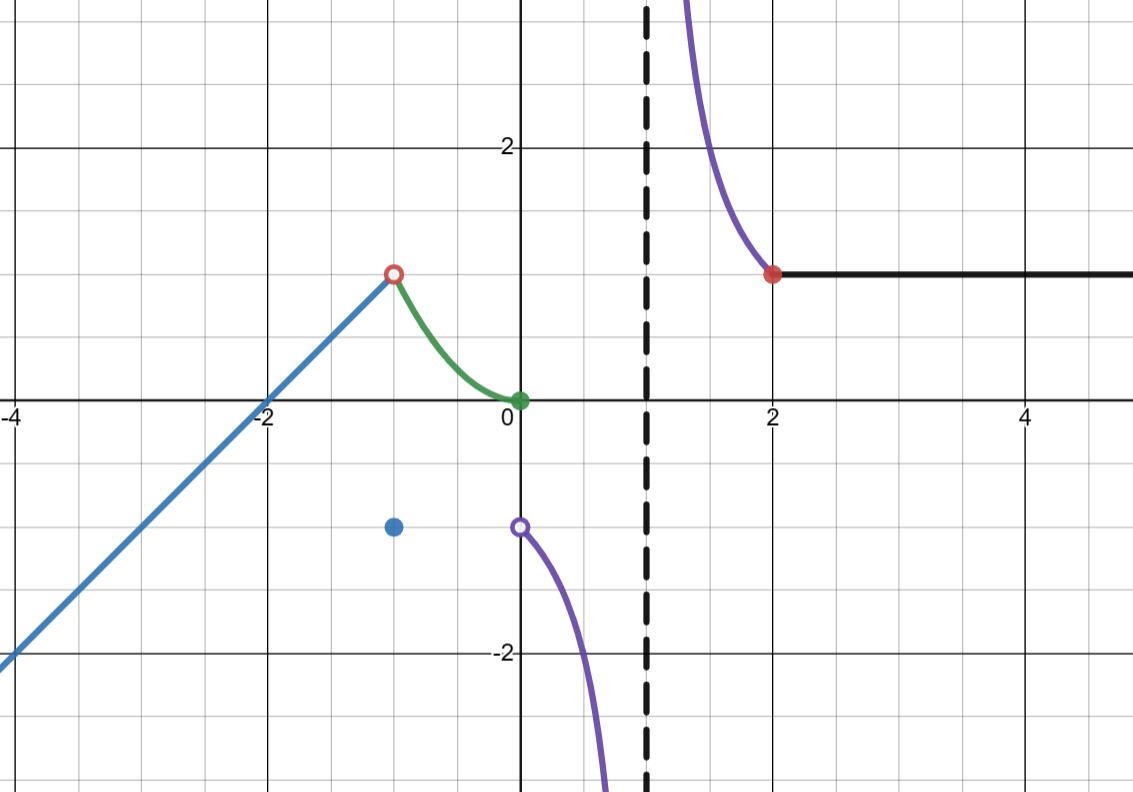
\includegraphics[scale=0.3]{Images/Sum23pmt1pic2.jpeg}
\end{center}
\vspace{0.25in}
\begin{enumerate}
\begin{multicols}{2}
\vspace{0.1in}
\item $\displaystyle\lim_{x\to -1^{-}} f(x)$
\vspace{0.35in}
\item $\displaystyle\lim_{x\to -1^{+}} f(x)$
\vspace{0.35in}
\item $\displaystyle\lim_{x\to -1} f(x)$
\vspace{0.35in}
\item $f(-1)$
\vspace{0.35in}

\item $\displaystyle\lim_{x\to 0} f(x)$
\vspace{0.35in}
\item $\displaystyle\lim_{x\to 1^-} f(x)$
\vspace{0.35in}
\item $\displaystyle\lim_{x\to 1^+} f(x)$
\vspace{0.35in}
\item $\displaystyle\lim_{x\to 2} f(x)$
\vspace{0.35in}

\end{multicols}

\item Give the $x$-values where the function $f(x)$ is discontinuous.
\vfill
\item For the removable discontinuity/discontinuities, how can you redefine $f(x)$ to make it continuous there?
\vfill
\end{enumerate}
\pagebreak

\item For this problem, we're going to use the function $f(x) = \sqrt{x+3}$.
\begin{enumerate}
\item Compute the derivative using the definition of the derivative.
\vspace{4in}

\item What is the domain of $f$? What is the domain of $f'$?
\vspace{1in}
\item What is $f'(6)$?
\vspace{0.5in}

\item What is the equation of the tangent line of $f(x)$ at $a=6$?
\end{enumerate}
\end{enumerate}
\end{document}